\chapter[A revised notion of classicality \\ Spekkens non-contextuality]{A revised notion of classicality \\ \huge{Spekkens non-contextuality}}
\lhead{\emph{Spekkens non-contextuality}}
\label{sec:spekkcont}
\section{Outcome determinism for unsharp measurements (ODUM)}
\label{sec:odum}
We want a notion of classicality that accomodates unsharp measurements and is robust to noise. A first approach, assuming the validity of quantum theory, might entail simply extending KS non-contextuality to general POVM measurements, in the sense that a classical HVM assigns a conditional probability in $\{0,1\}$ to all positive semi-definite operators, such that for every resolution of the identity only one operator receives the valuation $1$. This incremental approach has been given the name ``ODUM", which stands for ``outcome determinism for unsharp measurements". The problem with ODUM is that it runs into numerous inconsistencies, as convincingly argued in \cite{Spekkens2014}. We confine ourselves to the most immediate inconsistency: Consider the quantum experiment consisting of an experimenter repeatedly performing the trivial POVM $\{\frac{\mathbb{1}}{2},\frac{\mathbb{1}}{2}\}$ on some arbitrary preparation $\rho$. Any classical value assignment to positive semi-definite operators would be in conflict with the normalization conditions for general ontological models in Section \ref{sec:hvm}, i.e.\ either the added probabilities of the two outcomes would be zero or exceed one. Thus, either this trivial POVM is non-classical according to the new notion, or the new notion is not meaningful. The trivial POVM corresponds to a fair coin flip - it can be implemented by simply throwing away the system and generating a random bit. Such a ``measurement" should by all means be considered classical. For this implementation, the only sensible choice is to assign every every ontic state $\lambda$ the conditional probability $\frac{1}{2}$, as measurement and system are completely decoupled. The same line of reasoning leads to the conclusion that the approach in Section \ref{sec:cswhierarch} cannot be extended to general unsharp measurements, as this produces inconsistencies when treating QM.

\section{Operational approach due to Spekkens}
\label{sec:spekkensopappr}
The previous examples highlight the need for a new notion of contextuality that captures the spirit of KS non-contextuality, but is applicable to realistic experimental scenarios. Let us take a step back and identify common features of the contextuality scenarios discussed so far, which led to behaviour we deemed non-classical. The setting was in all cases for the most part identical: we considered sets of projective measurements, with the key property that a given projector was shared amongst multiple measurements. Identical projectors appearing in multiple measurement contexts was crucial for proving a contradiction. Spekkens' approach captures this key feature and operationalizes the assumption. In QM, a positive semi-definite operator defines an operational equivalence class, in the sense that all measurement events which are operationally indistinguishable, for all states, must be represented by the identical operator. An analogous observation applies to density operators describing the preparation of a system.
On that account, instead of assuming a projector to be part of several measurements, Spekkens assumes certain measurement events to be operationally equivalent; we will formalize this shortly. Assuming KS non-contextuality, the implication of a projector appearing as part of multiple measurements is that it must be assigned the same conditional probability $\{0,1\}$ by the ontological model, for all ontic states $\lambda$. In other words, operationally equivalence implies an identical ontological representation. We will find that Spekkens' revised notion of non-contextuality follows exactly this prescription.  

In \cite{Spekkens2005}, Spekkens introduces a largely operational notion of contextuality for preparations, measurements, and transformations. It is a revision of KS contextuality that addresses several shortcomings of the traditional definition. Contextuality is generalized to apply to arbitrary operational theories. In comparison, KS contextuality is limited to the scope of QM, as it is defined within the framework of quantum theory. Furthermore, the revised definiton will not assume outcome determinism at an ontic level, accomodating HVM whose indicator functions are more general mappings $\Lambda\mapsto [0,1]$. Taking QM as operational theory, Spekkens contextuality extends to arbitrary measurements, including physical, non-projective ones. In fact, within the Spekkens framework, measurements, preparations, and transformations can be considered black box devices, i.e.\ primitives of which one can compose an experiment. An operational theory makes predictions about these operational primitives, i.e.\ assigns probabilities to measurement outcomes that are consistent with experimental observations. In QM, for instance, outcome probabilities are given by the Born rule, where we posit that every preparation is operationally fully specified by a density operator and every measurement by a POVM. A Spekkens non-contextual operational theory is one that is compatible with a Spekkens non-contextual ontological model, which we will define shortly. Spekkens' revised concept of non-contextuality will serve as a new, more suitable notion of classicality that is in particular compatible with unsharp measurements.

This section only discusses Spekkens non-contextuality for preparations and measurements, as transformations will not be relevant to our discussion\footnote{Consider a prepare-and-measure type experiment that consists of an initial state preparation, followed by some transformation of the system, and finally a measurement. We may consider the transformation as part of the initial preparation procedure, or as part of the final measurement, and describe the experiment solely in terms of preparation procedures and measurements.}. Preparations and measurements will be represented as outlined in Section \ref{sec:hvm}. In the following, if not states otherwise, the term ``contextuality" and all variant forms will refer to Spekkens contextuality.

The essence of what it means for an ontological model to be non-contextual can be summarized as follows:
An ontological model of an operational theory is \emph{non-contextual} if:
The operational equivalence of two experimental procedures, i.e.\ two preparations or two measurements, 
implies that they have an equivalent representation in the ontological model.
Two experimental procedures are operationally equivalent if they cannot be distinguished by any measurement statistics. 

Let us formalize the above, starting with preparation non-contextuality. We can define an equivalence relation on the set of all preparation procedures $P$ that partions the set into operational equivalence classes $[P]$. By the guiding principle above, we require equivalent preparations to have the same ontological representation in a non-contextual HVM.

\begin{definition}[\cite{Spekkens2005}]\hfill\break
\label{def:prepnc}
Two preparation procedures $P,P'$ are \emph{equivalent}, denoted $P\sim P'$, if 
\begin{equation*}
    \forall \text{ measurements } M,\thinspace \forall \text{ measurement outcomes } k\thinspace:\thinspace p(k\vert P,M)=p(k\vert P',M)\thinspace.
\end{equation*}

An ontological model is \emph{preparation non-contextual} if equivalent preparations have identical associated probability density functions on the ontic state space: 
\begin{equation*}
    \forall \text{ preparations } P\thinspace:\thinspace \mu_{P}=\mu_{[P]}\thinspace.
\end{equation*}
\end{definition}

Measurement non-contextuality is defined in an analogous manner:

\begin{definition}[\cite{Spekkens2005}]\hfill\break
\label{def:mntnc}
Two measurement procedures $M,M'$ are \emph{equivalent}, denoted $M\sim M'$, if their outcomes can be associated one-to-one and 
\begin{equation*}
    \forall \text{ outcomes } k\thinspace,\thinspace \forall \text{ preparations } P\thinspace:\thinspace p(k\vert P,M)=p(k\vert P,M')\thinspace.
\end{equation*}

An ontological model is \emph{measurement non-contextual} if equivalent measurements have identical associated indicator functions: 
\begin{equation*}
    \forall \text{ measurements } M\thinspace,\thinspace \forall \text{ outcomes } k\thinspace:\thinspace \xi_{M,k}=\xi_{[M],k}\thinspace.
\end{equation*}
\end{definition}

Spekkens proves three no-go theorems for ontological models of QM \cite{Spekkens2005}. These rule out preparation non-contextual, measurement non-contextual, and transformation non-contextual models, respectively. All three proofs apply to two-dimensional Hilbert spaces, making them stronger than traditional proofs of contextuality.

Whenever referring to a non-contextual ontological model, without specifying whether we are referring to preparations or measurements, we  will assume the ontological model to be both preparation and measurement non-contextual. As the reasons for assuming classical correlations to be compatible with a measurement non-contextual HVM description are the same as those for preparation non-contextuality, the combination of both is the only natural assumption of non-contextuality.

We now discuss to what extent non-contextuality is a sensible notion of classicality. A contextual ontological model implies a difference in reality that cannot be observed. Such a model is in conflict with Leibniz' ``Identity of Indiscernibles" \cite{Buchanan2019,Spekkens2019}. Leibniz's principle states that two empirically indistinguishable scenarios are to be ontologically equivalent. As such, it rejects ontological models for which there exist ontologically distinct, but empirically indistinguishable scenarios. Recall that, within QM, KS non-contextuality can be seen as a generalization of Bell's notion of local determinism to non-remote measurement contexts. One can also link Leibniz' principle, which is at the heart of Spekkens' revised notion of contextuality to Bell's notion of local causality. Like before, local causality is the weaker assumption, which is owed to the fact that Bell-type experiments impose additional constraints on the experiment's causal structure:

In principle, it might well be the case that an agent's free choice of measurement can have a causal influence on a remote system and alter the ontic or "matter of fact" state of that system. However, physicists have yet to devise an experiment producing correlations that are in conflict with the no-signalling principle, which is reinforced by special relativity. Therefore, to the best of our knowledge, such causal influence, if it exists, is not detectable. This in turn means that an agent in the remote frame of reference can detect no difference in the physical properties of his system for different free choices of measurement. Local causality is the assumption that there is in fact no difference at the ontic level, and thus provides the most natural explanation for our inability to detect a causal influence. Another, more hair-raising explanation could be that all possible ensemble preparations in principle accessible to an experimenter are too spread out to resolve minor differences in the conditional probabilities. The assumption of local causality just corresponds to Leibniz' principle applied to Bell-type experiments with space-like separated measurements. The assumption of Spekkens non-contextuality simply extends the applicability of Leibniz's principle to arbitrary prepare-and-measure type experiments, in particular those without remote subsystems.

Just as local causality is motivated by the no-signalling principle, local causality providing the most natural explanation for the impossibility of superluminal signalling, a point can be made that non-contextuality is perhaps equally well motivated by Leibniz' Identity of indiscernibles. Analogously to local causality, non-contextuality is the most natural explanation for operational equivalences. Spekkens points out that the credentials of Leibniz' principle parallel those of no-signalling and that it was critical in Einstein's conception of relativity \cite{Buchanan2019,Spekkens2019}. Take for instance the equivalence principle which states that one cannot distinguish between being at rest in a uniform gravitational field and accelerating uniformly through free space. Within Newtonian mechanics the two scenarios are ontologically distinct, as one's absolute acceleration differs in both cases. On his way to general relativity, Einstein reasoned that the empirical indistinguishablitiy of both scenarios implies that they should be treated as ontologically equivalent by a physical theory, a powerful invocation of Leibniz's principle that reshaped our perception of reality. An almost identical line of reasoning is found in Einstein’s 1905 paper ``On the electrodynamics of moving bodies" \cite{Einstein1905}. He notes that the predictions of Maxwell's equations depend only on relative motion. For example, the current induced in a coil will have the same magnitude and direction, no matter if we consider a magnet to be moving through the coil or the coil moving through the field of the magnet with equal but opposite velocity. To Einstein, this empirical indistinguishability was in conflict with the prevailing aether theories of the time. An aether would define a distinguished frame of reference, rendering the two empirically equivalent induction experiments ontologically distinct. Once again, Einstein's invocation of Lebniz' principle lead him to abandon aether theory and conceive relativity theory, in which both scenarios are equivalent.

In Section \ref{sec:spekkensineq} we will see how to lift KS non-contextuality inequalities to Spekkens non-contextuality inequalities by substituting assumptions about operator compatibility for assumptions about operational equivalence. Like before, these lifted non-contextuality inequalities, when violated, bear witness to the quantumness of the system, in the Spekkens sense. Violations of non-contextuality inequalities that prove nature's incompatibility with a non-contextual HVM description have been observed in experiments involving photonic qubit systems \cite{Mazurek2016}. While the lifted non-contextuality inequalities no longer make unphysical assumptions about the measurements themselves, they introduce two new practical complications: the issue of tomographic completeness, and that of exact operational equivalence. Experimental tests of non-contextuality inequalities assume that we can implement a tomographically complete (TC) set of measurements and state preparations. The reason for this is that, according to Definitons \ref{def:prepnc}, \ref{def:mntnc}, two experimental procedures can only be asserted operationally equivalent if the two procedures are operationally indistinguishable, for all possible prepare-and-measure-type experiment that utilize them. For instance, two preparations are only operationally equivalent if they produce the same statistics for all possible measurements, requiring in principle an infinite number of tests. In practice, we aim to identify a TC set of measurements, such that for an arbitrary measurement and preparation there is a functional relationship between the statistics of that measurement and those of the TC set. As such, if two preparations are operationally equivalent with respect to a TC set of measurements, they are operationally equivalent with respect to all measurements. Within QM, a TC set of measurements for a qubit system is given by the three Pauli measurements $\sigma_x$, $\sigma_y$, and $\sigma_z$, that together determine the three Bloch vector components of an arbitrary state. Problematically, without additional assumptions, we can in practice never declare a set of measurements to be TC. What we can do is try our best to refute such a claim. Additionally, there are tests of contextuality that account for some number of unknown measurements in a TC complete set \cite{Pusey2019a}. By implementing more preparations and measurements one can in principle account for an arbitrary number of unknown measurements in a TC set. We will make use of the results in \cite{Pusey2019a} in Section \ref{sec:protocols}, and they will allow us to relax the assumption of TC. Just like in the case of KS contextuality, where had to assume operator compatibility, we cannot expect to devise a fully device-independent self-testing protocol based on non-contextuality. 

Another issue with experimental tests of contextuality is that Definitions \ref{def:prepnc}, \ref{def:mntnc} assume exact operational equivalences, requiring infinite precision. This problem has been tackled in \cite{Pusey2018,Mazurek2016}. Let us for the moment consider operational equivalences amongst preparations. The key is noticing that performing measurements on some set of preparations defines the statistics for all preparations in the convex hull. As part of post-processing, we can define new preparations in the convex hull, whose statistics we know, and that are exactly operationally equivalent. The price to pay is that these new preparations may be less optimal than the original ones, in the sense that they may only produce a lesser violation of the non-contextuality inequality. This ``fitting" process that establishes exact operational equivalences is done within the framework of generalized probabilistic theories (GPT). Operational equivalences amongst measurements are treated in an analogous manner.

Finally, we wish to understand how KS contextuality and Spekkens contextuality are related. It turns out that a Spekkens non-contextual ontological model of QM assign deterministic outcomes to projective quantum measurements and induces a KS non-contextual outcome assignment, like in Definition \ref{def:kscontherm}, if we restrict measurements to projective ones. 
KS non-contextuality is an assumption that restricts the ontological representation of compatible (commuting) projective measurements. Let us therefore examine what conditions Spekkens non-contextuality imposes on the ontological representation of compatible measurements. Spekkens non-contextuality covers arbitrary, not necessarily sharp, measurements and applies to arbitrary operational theories. Therefore, recall Definition \ref{def:compat}, which defines what it means for two measurements to be compatible, purely in operational terms.

Let $M_{1}$ and $M_{2}$ be compatible measurements according to Definition \ref{def:compat}, and $M_{12}$ a dual outcome measurement that jointly realizes $M_1$ and $M_2$. By definition, the measurement procedure $M_{1}$ is operationally equivalent to measuring $M_{12}$ and discarding register two. Analogously, the measurement procedure $M_{2}$ is operationally equivalent to measuring $M_{12}$ and discarding register one. What can be said about the ontological representation of compatible measurements within a Spekkens non-contextual model? In a Spekkens non-contextual ontological model, operationally equivalent measurement procedures have identical associated indicator functions. For the measurements $M_{1}$, $M_{2}$, and $M_{12}$ like above, this implies:
\begin{align*}
\forall\thinspace\lambda\in\Lambda,\thinspace\forall \thinspace P,\thinspace\forall\thinspace a_{k}:p(a_{k}\thinspace\vert\thinspace M_{1},P,\lambda)=\sum_{b_{j}}p(a_{k},b_{j}\thinspace\vert\thinspace M_{12},P,\lambda)\\
\forall\thinspace\lambda\in\Lambda,\forall\thinspace P,\thinspace\forall\thinspace b_{k}:p(b_{k}\thinspace\vert\thinspace M_{2},P,\lambda)=\sum_{a_{i}}p(a_{i},b_{k}\thinspace\vert\thinspace M_{12},P,\lambda)
\end{align*}
Consequently, a Spekkens measurement non-contextual ontological model is one for which the probability of measuring say $M_{1}$ and obtaining the outcome $a_{k}$, conditioned on the system being in any ontic state, is independent of what other compatible measurements are simultaneously performed. If we consider QM as operational theory, this is the essence of KS non-contextuality, as discussed in Section \ref{sec:kscont}, with the notable difference that we have decoupled outcome determinism from context independence.

Interestingly, it can proven that a Spekkens non-contextual ontological model must fix the outcomes of sharp measurements deterministically \cite{Spekkens2014}. This result is robust, in the sense that ``almost sharp" measurements are assigned outcomes ``almost deterministically". Thus, for projective measurements, the notion of Spekkens non-contextuality reduces to KS non-contextuality. For Spekkens non-contextual ontological models, outcome determinism for sharp measurements can thus be derived from within the framework itself, and is not an assumption introduced ad-hoc, as was the case for KS non-contextuality.

\section[Spekkens non-contextuality inequalities \\ KCBS revisited]{Spekkens non-contextuality inequalities \\ \large{KCBS revisited}}
\label{sec:spekkensineq}

As before, let $n\geq 5$ be an odd integer.
In Section \ref{sec:csw} we saw that $n$ measurement events obeying cyclic exclusivity, in the sense that $p(\epsilon_i)+p(\epsilon_{i\oplus 1})\leq 1$ for all preparations $P$, give rise to a linear combination of probabilities, $S=\sum_{i=1}^n p(\epsilon_i)$,
such that for all deterministic assignments of probabilities to the measurement events that respect these exclusivity relations, the value of $S$ is upper bounded by \ref{eqn:ncycleideal}.
Furthermore, we found that there exist quantum models, involving $n$ projective measurements on the initial qutrit state $\ket{0}$, that respect cyclic exclusivity (orthogonality) but violate this bound.
The important thing to remember is that a key ingredient in deriving these KS non-contextuality inequalities was outcome-determinism, i.e.\ the assumption that the ontological model's indicator functions induce a deterministic outcome assignment. While the assumption of outcome-determinism is baked into the framework of KS non-contextuality, Spekkens non-contextuality decouples the assumption of context-independence from that of outcome-determinism. If we relax outcome-determinism, then the class of inequalities in Section \ref{sec:kcbs} no longer delimit classical from quantum correlations, as we saw in Section \ref{sec:cswunsharp}. We now discuss how to lift the odd $n$-cycle KS non-contextuality inequalities to Spekkens non-contextuality inequalities that apply to general ontological models.

For KS scenarios with sharp measurements, we found measurement events obeying cyclic exclusivity, in the sense that $p(\epsilon_i)+p(\epsilon_{i\oplus 1})\leq 1$, by assuming cyclic compatibility relations for the $n$ measurement operators. This implied joint measurability of $M_i$ and $M_{i\oplus 1}$, and we considered measurement events arising from two sequential measurements. Two such measurement events that featured different outcomes for an identical measurement were defined as exclusive and associated with orthogonal projectors. Since these exclusive events could be perfectly distinguished by a single subsequent measurement, the sum of their probabilities was bounded by 1.
This time around, since we want to replace assumptions about operator commutativity and sharpness with operational equivalences, we establish the exclusivity of two measurement events by associating them with distinct outcomes of a single measurement:
Consider a measurement $M_i$ with the three outcomes $m_1$, $m_2$, and $m_3$. As $m_k$ and $m_l$, for $k\neq l$, are two distinct outcomes of a single measurement $M_i$, we immediately obtain the exclusivity constraint $p_{m_k\vert M_i}+p_{m_l\vert M_i}\leq 1$. We now sketch how to construct say $n=5$ measurement events satisfying cyclic exclusivity, consistent with the KCBS scenario \cite{Kunjwal2019}.
We take the ideal reference experiment \ref{eqn:ncycleideal} involving a qutrit system as blueprint. Due to cyclic compatibility, each cycle state $\vert u_i^{(n)} \rangle$ can be extended to an orthogonal triad that contains $\vert u_{i\oplus 1}^{(n)} \rangle$, or to an orthogonal triad that contains $\vert u_{i\oplus (n-1)}^{(n)} \rangle$. Since these triads resolve the identity, the ideal rank one projectors belonging to such orthogonal triad can be seen as the elements of a single three-outcome POVM. When considering the ideal case, we can alternatively think of these as projectors onto the one-dimensional eigenspaces of some Hermitian measurement operator acting on the qutrit space.

So far, we have discussed the KCBS scenario only in terms of binary measurements. By relating the ideal reference experiment to a set of three-outcome measurements performed on a qutrit allows us to implement exclusivity constraints via operational equivalences: Let $\{M_i\}_{i=1}^n$ be $n$ three-outcome measurements with outcomes labeled $m_1$, $m_2$, and $m_3$, reminiscent of the ideal measurements we just constructed. Further assume that we perform the measurements on some distinguished preparation $P_0$ and determine the value of the linear combination $R=\sum_{i=1}^n p(m_1\thinspace \vert \thinspace M_i,P_0)$.
If we assume the measurement events $m_3 \thinspace \vert \thinspace M_i$ and $m_1 \thinspace \vert \thinspace M_{i\oplus 1}$ to be operationally equivalent for all $i\in\{1,\dots,n\}$,  $m_3 \thinspace \vert \thinspace M_i \equiv m_1 \thinspace \vert \thinspace M_{i\oplus 1}$, then we obtain $n$ measurement events $\{m_1\vert M_i\}_{i=1}^n$ that obey $p(m_1\vert M_i)+p(m_1\vert M_{i\oplus 1})\leq 1$ for all $i$. The measurement events are depicted in Figure \ref{fig:kcbsspekkens}. 

\begin{figure}
	\begin{subfigure}[t]{0.45\textwidth}
    	\centering
    	\includegraphics[width=\textwidth]{images/kcbsspekkens.png}
        \caption{}
	\end{subfigure}
	\hfill
    \begin{subfigure}[t]{0.45\textwidth}
    	\centering 
        \includegraphics[width=0.8\textwidth]{images/kcbsrefstates.png}
        \caption{}
    \end{subfigure}
    \caption{\textbf{(a):} Schematic depicting the prepare-and-measure scenario assumed for lifting the odd $n$-cycle KS non-contextuality inequalities to Spekkens non-contextuality inequalities. The scenario consists of $n=5$ three-outcome measurements $M_i$, with outcomes $m_1$, $m_2$, and $m_3$, as well as $3n$ preparations $\{P_{m_k\vert M_i}\}_{k,i}$, a distinguished preparation $P_0$, and two auxilliary preparations $P_1$, $P_2$. The measurement events $m_3\thinspace\vert\thinspace M_i$ and $m_1\thinspace\vert\thinspace M_{i\oplus 1}$ are overlapping, to highlight the fact that we assume operational equivalence $m_3\thinspace\vert\thinspace M_i\equiv m_1\thinspace\vert\thinspace M_{i\oplus 1}$. The $S_i$ are convex combinations of the preparations $\{P_{m_k\vert M_i}\}_k$, $S_i\equiv \sum_k p_k^{(i)}P_{m_k\vert M_i}$. $S_0$ is a convex combination $S_0=\sum_j p_j^{(0)}P_j$ with $p_0^{(0)}>0$. The $S_i$ and $S_0$ are cocyclic to signify operational equivalence. Figure adapted from \cite{Kunjwal2019}. \textbf{(b):} Juxtaposition with the cycle states \ref{eqn:ncycleideal} belonging to the odd $n$-cycle scenario for $n=5$. Three-outcome measurements like in (a) can be constructed from the $n$ cycle-states $\{\vert u_i^{(n)}\rangle\}_i$ by extending each cycle state to an orthogonal triad $\subset \mathbb{C}^3$, and identifying each corresponding rank-one projector with an outcome of the measurement $M_i$. As the cycle-states obey cyclic orthogonality, we can construct measurements $M_i$ that satisfy the operational equivalences in (a).}
\label{fig:kcbsspekkens}
\end{figure}

Imposing the operational equivalences $m_3\thinspace \vert \thinspace M_i\equiv m_1\thinspace \vert \thinspace M_{i\oplus 1}$, any Spekkens non-contextual ontological model must assign the same probability to the equivalent measurement events $m_3\thinspace \vert \thinspace M_i$ and $m_1\thinspace \vert \thinspace M_{i\oplus 1}$, for all ontic states $\lambda\in\Lambda$. In other words, an event must be assigned the same probability for all ontic states, no matter what measurement it is a part of. If we could justify imposing outcome-determinism on all indicator functions associated with the $n$ measurements $\{M_i\}_{i=1}^n$ on the support of the preparation $P_0$, i.e.\ the subset $\Lambda_0\subset\Lambda$ of ontic states for which $p(\lambda\vert P_0)>0$, then the Spekkens non-contextual bound on the linear combination $S$ corresponds to just the KS non-contextual bound. 
To this effect, \cite{Kunjwal2019} introduces a new operational quantity which measures the  predictability of the measurements $M_i$. For some set of preparations $\{P_{m_k\vert M_i}\}$, $k\in\{1,2,3\}$ and $i\in\{1,\dots,n\}$, \cite{Kunjwal2019} defines
\begin{equation}
\text{Corr} = \sum_i q_i \sum_{k} p_k^{(i)} p(m_k \thinspace\vert\thinspace M_i, P_{m_k\vert M_i}),
\end{equation}
where $\{q_i>0\}_i$ is an arbitrary probability distribution, such that the maximum algebraic value of $\text{Corr}$ is $1$. The $\{p_k^{(i)}\}_k$ are also probability distributions, but require further explanation:
Take QM as operational theory. In the ideal case, for noise-free measurements and preparations, we find and may prepare $P_{m_k\vert M_i}$ such that $\text{Corr}=1$ (denote by $P_{m_k\vert M_i}$ the pure state preparation corresponding to the rank-one projector $m_k\thinspace\vert\thinspace M_i$). If $\text{Corr}=1$, we know that the measurements $M_i$ act in deterministic fashion on the convex combination $S_i \coloneqq \sum_k p_k^{(i)} P_{m_k\vert M_i}$ and a valid ontological model must be deterministic, at least for all ontic states in the support of $S_i$. Assume that we can find distributions $\{p_k^{(i)}\}_k$, such that $S_i\equiv S_0$, where $S_0$ is some convex combination of preparations, containing $P_0$ with weight $p_0>0$. We may infer from operational equivalence that the preparations $S_i$ and $S_0$ have identical support, and in particular that the measurements act in deterministic fashion also on the preparation $S_0$, and by extension $P_0$. The distributions $\{p_k^{(i)}\}_k$ in the definition of $\text{Corr}$ are distributions that establish the operational equivalences above. In the case of noise-free measurements, $\text{Corr}=1$, we conclude that the Spekkens non-contextual upper bound of the linear combination $R=\sum_{i=1}^n p(m_1\thinspace\vert\thinspace M_i,P_0)$ coincides with the Kochen-Specker bound \ref{eqn:oddncycleclass} of the odd $n$-cycle inequality. Thus, by considering also correlations between preparations and measurements, we can witness Spekkens non-contextuality. Of course, for physical implementations of the experiment, we will always observe $\text{Corr}<1$. The remarkable thing, proved in \cite{Kunjwal2019}, is that there is a trade-off between the minimal value of $R$ one must observe to witness Spekkens contextuality and the amount of noise in preparations and measurements that renders the measurements not perfectly deterministic. For $n=5$, the following is a Spekkens non-contextuality, reminiscent of the KCBS KS non-contextuality inequality:
\begin{equation}
R\leq 2+\frac{1-\text{Corr}}{p_0},
\end{equation}
where $2$ is the KS bound on the sum of five measurement events obeying cyclic compatibility, and $p_0$ is the weight of the distinguished preparation $P_0$ in the convex combination $S_0\equiv S_i$.

In the ideal case and assuming quantum mechanics as operational theory, we may construct operationally equivalent $S_i$, $S_0$ by setting $p_k^{(i)}=\frac{1}{3}$ and choosing for $S_0$ the convex combination with equal weights of $P_0$ and two pure state preparations in an orthogonal triad. This results in $S_0 \equiv \frac{\mathbb{1}}{3} \equiv S_i$.
On a final note, as proved in \cite{Kunjwal2019}, these lifted inequalities are not violated by trivial POVM, as was the case for the original KS non-contextuality inequalities, see Section \ref{sec:cswunsharp}.

We will make use of these lifted Spekkens non-contextuality inequalities in Section \ref{sec:relaxmemoryass}, as an alternative method of certifying quantumness.